\section{Requirements}

All building blocks in this thesis are developed with the purpose in mind to give the user the possibility to visualize and interact with complex 2D and 3D data, while being able to easily extend the library.
To enable this kind of functionality, a lot of parts of the infrastructure need to work seamlessly together.
Certain design choices had to be made to guarantee this. As speed is the most constraining factor, this chapter will start by introducing the design choices that had to be made in order to achieve state of the art speed.

\vspace{1em}
\begin{minipage}{\linewidth}
    \centering
    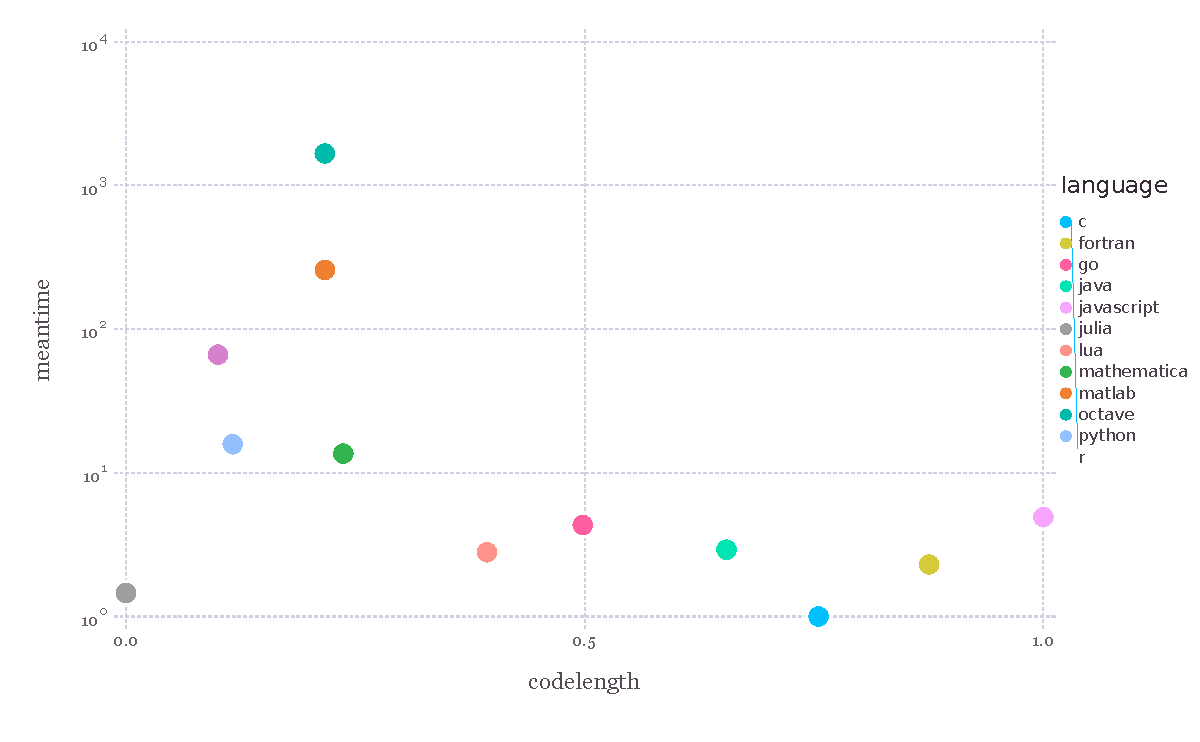
\includegraphics[width=0.9\linewidth]{graphics/julia_bench.pdf}
    \captionof{figure}[Volume Visualization]{Languages speed relative to C (averaged benchmark results), plotted against the length of the needed code (Source in Appendix).}
    \label{fig:juliabench}
\end{minipage}


\subsubsection{Speed}
Speed is mainly a usability factor. It is a factor, that can make a software unusable, or render it unproductive. Because of this, speed has taken a high priority in this thesis. As general coding productivity is also a concern, this thesis is set on using a high level language.
Historically, these two demands can not be satisfied at the same time.
How to achieve state of the art speed with a high level language is an ongoing research and basically the holy grail of language design. 
Julia promises to do exactly this, which is illustrated in figure \ref{fig:juliabench}. 
Code length is an ambiguous measure for conciseness, but if the code is similarly refactored it is a good indicator of how many lines of code are needed to achieve the same goal.
From this figure we can conclude, that Julia at least comes close to its promises, which is why it has been chosen as the programming language.

To get high performant 3D graphics rendering, there are on the first sight a lot of options.
If you start to take the previous demands into account, the options shrink down considerably.
The visualization library should be implemented in one high level language, which can be used for scientific computing and has state of the art speed. 
At this point, there are close to zero libraries left. As you can see in figure \ref{fig:juliabench}, Matlab, Python and R disqualify, as they are too slow. JavaScript, Java, Go and Lua are missing a scientific background and the others are too low level for the described goals.
This leaves only Julia, but in Julia there were no 3D libraries available, which means that one has to start from scratch.
There are only a couple of GPU accelerated low-level libraries available, namely Khrono's \ac{OpenGL}, Microsoft's DirectX, Apple's Metal and AMD's Mantel, which are offering basically the same functionality. 
As only \ac{OpenGL} is truly cross-platform, this leaves \ac{OpenGL} as an option.
So for the purpose of high speed visualizations, \ac{OpenGL} was wrapped with a high-level interface written in Julia. This leaves us with one binary dependency not written in Julia, namely the video driver, which implements \ac{OpenGL}.

Measurement of success is pretty straight forward, but the devil is in the detail.
It is easy to benchmark the code, but quite difficult to find a baseline, as one either has to implement the whole software with an alternative technologies, or one has to find similar software.
This thesis will follow a hybrid strategy, comparing some simple implementations with different technologies and choose some rivaling state of the art libraries as a baseline.

\subsubsection{Extensibility}
Extensibility is an important factor, which can decide, if a library is fit for scientific computing or not. 
It is not only that, but also a great factor determining growth of a software, as the more extensible the software is, the higher is the probability that someone else contributes to it.
In order to write extensible software, we first have to clarify what extensibility is.
Extensible foremost needs that the code is accessible. There are different levels of accessibility. The lowest level is closed source, where people purposely make the code inaccessible. While this is obvious, it is just a special case of not understanding the underlying language. Just shipping binaries without open sourcing the code, means that the source is only accessible in a language which is extremely hard to understand, namely the machine code of the binary. So another example for inaccessibility is to write in a language that is difficult to understand. Other barriers are obfuscated language constructs, missing documentations and cryptic highly optimized code.
Further more the design of the library in the whole is an important factor for extensibility. It is not only important, that all parts are understandable, but also, that every independent unit in the code solves only one problem. This guarantees that one can quickly exchange it, or use it somewhere else where the same problem needs to be solved.
If this is guaranteed, re-usability in different contexts becomes much simpler. This allows for a broader user base, which in turn results in higher contributions and bug reports.
Short concise code is also important, as it will take considerably less time to rewrite something, as the amount of code that has to be touched is shorter and less time is spend on understanding and rewriting the code.

So the code written for this thesis will be open source, modular, written in a high level language and concise.

This is pretty difficult to measure as these are either binary choices, which are followed or not, 
or higher level concepts like writing concise code, which can be a matter of taste.
To get an idea of the effectiveness of the strategy, usage patterns and feedback from Github will be analyzed.

\subsubsection{Event System}
The event system is a crucial part of the library, as the proclaimed goal is to visualize dynamic, animated data.
This means, there are hard demands for usability and speed on the event system.
The chosen event system has an immediate influence on how to handle animations. 
This lead to the design choice of using signals. Signals are a very good abstraction for values that change over time.
If well implemented, it makes it natural to reason about time, without the need of managing unrelated structures and callback code.

\subsubsection{Interfaces}

Working with a computer means working with interfaces to a computer, which in the end simply juggles around with zeros and ones. There is a huge hierarchy of abstractions involved, to make this process of binary juggling manageable to the human.
We already dealt with the lowest relevant abstraction: the choice of programming language, which forms our first interface to the computer.
The next level of abstraction is the general architecture of the modules, which has been discussed previously. 
This chapter is about the API design choices that have been made.

The first API is the \ac{OpenGL} layer. 
The philosophy is to make the wrapper for native libraries as thin and reusable as possible and an one to one mapping of the underlying library.
This guarantees re-usability for others, as they might be used to work only with the low-level library or they might disagree with some higher-level abstraction and prefer to write their own.

Over this sits an abstraction layer needed to simplify the work with \ac{OpenGL}.
With this abstraction, the actual visualization library is implemented.

\ac{API}s for visualization libraries are very difficult to realize, as there are endless ways of visualizing the same data.
The design choice here was to use Julia's rich type system to better describe the data. 
Julia makes this possible, as you can create different types for the same data, without loosing performance.
So you can have a unit like meters represented as a native floating point type and have the visualization specialize to this.
Like this you can have a single function e.g. \textit{visualize}, that does create a default visualization for different data types. Instead of manually passing additional information to the visualization function, it is coded in the type itself.
Together with the event system which consists of signals, it is possible to edit and visualize rich data over a simple interface, which is perfect for visual debugging, as it is always the same function call applied to the data and no further user interaction is needed.
It is also easy to extend, as the user just has to overload the function with a custom style and optional key word arguments.
Finally, there are also graphical user interfaces developed for this thesis. As also optimizing them is out of the scope of this thesis, they are kept very simple.
The measurement of success is again relatively difficult to do. (I need to think this over)







\section{Used Technologies}

\subsection{The Julia Programming Language}
The basic introduction of Julia has already been given in the Background chapter.
This chapter is focused on how to write programs with Julia.
Most influential language construct are its hierarchical type system and multiple dispatch.
Multiple dispatch is in its core function overloading at runtime. 
To better understand multiple dispatch, one has to be familiar with Julia's type system.
The type system builds upon four basic components. 
Composite types, which are comparable to C-Structs, parametric composite types, bits types, abstract and parametric abstract types.
While the first three are all concrete types, abstract types can not be instanciated but are used to build a type hierarchy.
Every concrete type can only inherit from one abstract type, while abstract types can also inherit from abstract types.
Bit types are just immutable, stack allocated memory chunks, usable for implementing numbers.
You can build type hierarchies like this:
\begin{lstlisting}
abstract Number
abstract FloatingPoint{Size} <: Number # inherit from Number
bitstype 32 Float32 <: FloatingPoint{32} # inherit from a parametric abstract type
type Complex{T} <: Number
    real::T
    img::T
end
\end{lstlisting}

With this type hierarchy you can overload functions with abstract, concrete or untyped arguments.

\begin{lstlisting}
foo{T}(y::Complex{T}, y::Float32) = println("some number: ", x, " some complex Number: ", y) # shorthand function definition
function foo(x)
    println("overloading foo with a new unspecific signature")
end
\end{lstlisting}

What will happen at runtime is, that Julia compiles a method specialized on the arguments which results in overloading the function with the concretely typed arguments.
To illustrate this let us look at the example. 
Initially, foo will be overloaded with two methods.
Now, if you call foo with one Float32 argument, a new method will be added at run time specialized to Float32.
Like this, if the function does not access non constant global values, all types inside the function will be known at call time.
This allows Julia to statically compile the function body, while propagating the type information down the call-tree.

With multiple dispatch, Julia is definitely a functional oriented language. But there are also ways to give Julia a more object oriented feel.
Functions are first-class, so they are easy to pass around. 
They can be bound to variables and can then be called like normal functions via the variable name. This implies that functions can also be bound to objects.
There is no self reference available in Julia, so the object still needs to be passed to function via the function arguments

Another of the most crucial features is the very simple, overhead less C-Interface. 
Thanks to the binary compatibility of LLVM's emitted assembly, a C function call to a shared library inside Julia has the same overhead as it would be from inside C\cite{CCALL}. 
This is perfect for dealing with low-level libraries like \ac{OpenGL} and \ac{OpenCL}.


\subsection{\ac{OpenGL}}

\vspace{1em}
\begin{minipage}{\linewidth}
    \centering
    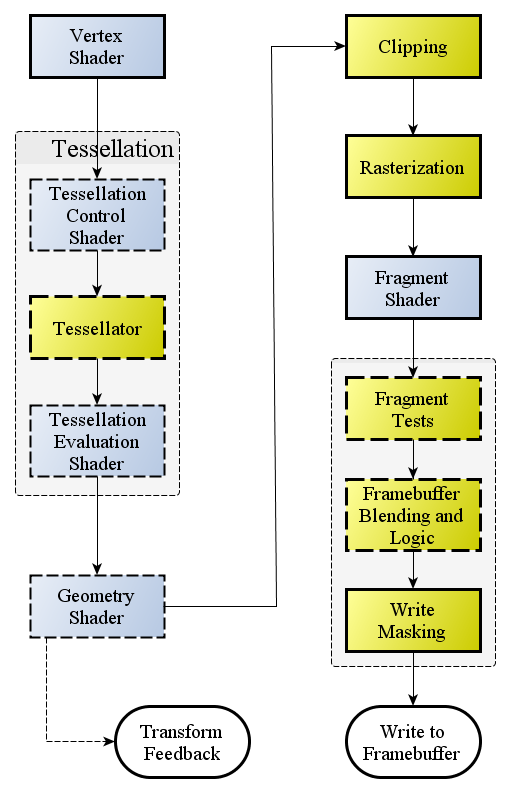
\includegraphics[width=0.5\linewidth]{graphics/RenderingPipeline.png}
    \captionof{figure}[OpenGL]{Diagram of the Rendering Pipeline. The blue boxes are programmable shader stages. Arrows show the flow of data\cite{OpenGLPipeline}}
    \label{fig:opengl}
\end{minipage}


\ac{OpenGL} is a low-level graphics API implemented by the video card vendor via the video driver. 
As such it does not offer much abstraction over the actual \ac{GPU}, but instead offers high flexibility and performance.
\ac{OpenGL} 1.0 was released in 1992 and the current version is 4.5.
A critical element when developing \ac{OpenGL} applications is, that not all video drivers implement the newest \ac{OpenGL} standards.

As a result, one has to decide which \ac{OpenGL} version to program against, trading between modernity and platform support.
For Romeo, it was decided to support \ac{OpenGL} 3.3 as the lowest bound, as it is sufficiently available, while still having most of the modern features.
The features include instance rendering, vertex arrays and modern \ac{GLSL} shader.

In figure \ref{fig:opengl} you can see the basic architecture of an OpenGL program pipeline.
As the description states, the blue boxes are programmable shaders, while the dotted boxes are optional parts of the pipeline.
The yellow boxes describe stages which are not directly accessible. They are part of the global OpenGL state, which can be set via OpenGL commands.

So in order to have a functioning OpenGL rendering pipeline one just needs to write a vertex shader and a fragment shader.
All shaders are compiled and linked into a program object, which then can be executed on the \ac{GPU}.
Shaders are written in a C dialect specialized for vector operations. 
You feed shaders with data via buffers, textures and uniforms. Buffers are 1D arrays, textures 1D/2D/3D arrays with both having their own memory, while uniforms live in the program object.

The different shaders are used to apply geometric, perspective transforms and calculating the light.
In newer APIs general compute operations are available, making it possible to create more flexible shaders.
Finally, the fragment shader rasterizes the data to the screen.
Here is a simple minimal example for a program rendering some vertex data with a flat color to the screen.

\begin{lstlisting}
//Vertex Shader
in vec3 vertex; // vertex fed into the shader via a buffer
uniform mat4 projection; // Projection matrix
uniform mat4 view; // View matrix, setting rotation and translation of the camera
void main()
{
    gl_position = projection*view*vec4(vertex, 1); // apply transformations to vertex and output to fragment shader
}
//Fragment shader
out vec4 framebuffer_color; //output from fragment shader, which will get written into the display framebuffer
void main()
{
    framebuffer_color = vec4(1,0,0,1); // write a red pixel at gl_position from the vertex shader.
}
\end{lstlisting}

All visualization code is written in OpenGL shaders, which get compiled and called via GLAbstraction.



\subsection{Reactive}
Reactive\cite{Reactive} is a functional event system designed for event driven programming.
It implements Elm's\cite{Elm} signal based event system in Julia.
Signals can be transformed via arbitrary functions which in turn create a new signal.
This simple principle leads too a surprisingly simple yet effective way of programming event based applications.

\begin{lstlisting}
a = Input(40)       # an integer signal.
b = Input(2)        # an integer signal.
c = lift(+, a,b)    # creates a new signal with the callback plus. Equal to c = a+b
lift(println, c)    # executes println, every time that c is updated. 
push!(a, 20)        # updates a, resulting in c being 22
#prints: 22
push!(b, 5)         # updates a, resulting in c being 22
#prints: 25
\end{lstlisting}

Lifting a signal creates a callback, which gets called whenever the signal changes.
There are more operations than lifting, like folding, merging, filtering and so on.
With this, one can build up a complex tree of operators which will get applied to the origin signal.
For the concrete case of Reactive, every signal carries around a list of children and parents.
Each signal has a rank, in order to build up a sorted heap with these information.
So every time a signal is updated, the heap can be traversed and the functions get applied in the right order, updating all the values of the children.
Reactive is used in all parts of the library. It builds the basis for the camera code, the widgets and any value that needs to be animated is realized via a signal.

\subsection{GLFW}
GLFW\cite{GLFW} is a cross platform \ac{OpenGL} context and window creation library written in C.
GLFW allows to register callbacks for a multitude of events like keyboard, mouse and window events.
This, together with a wrapper library for Julia makes GLFW perfect for doing the window creation.
In addition, GLFW exposes low level features like the operating systems context handle.
This can be used for creating advanced contexts that share memory with another context.
Romeo does not use this feature yet, but it makes GLFW a future proof choice.


\section{Implementation}

\vspace{1em}
\begin{minipage}{\linewidth}
    \centering
    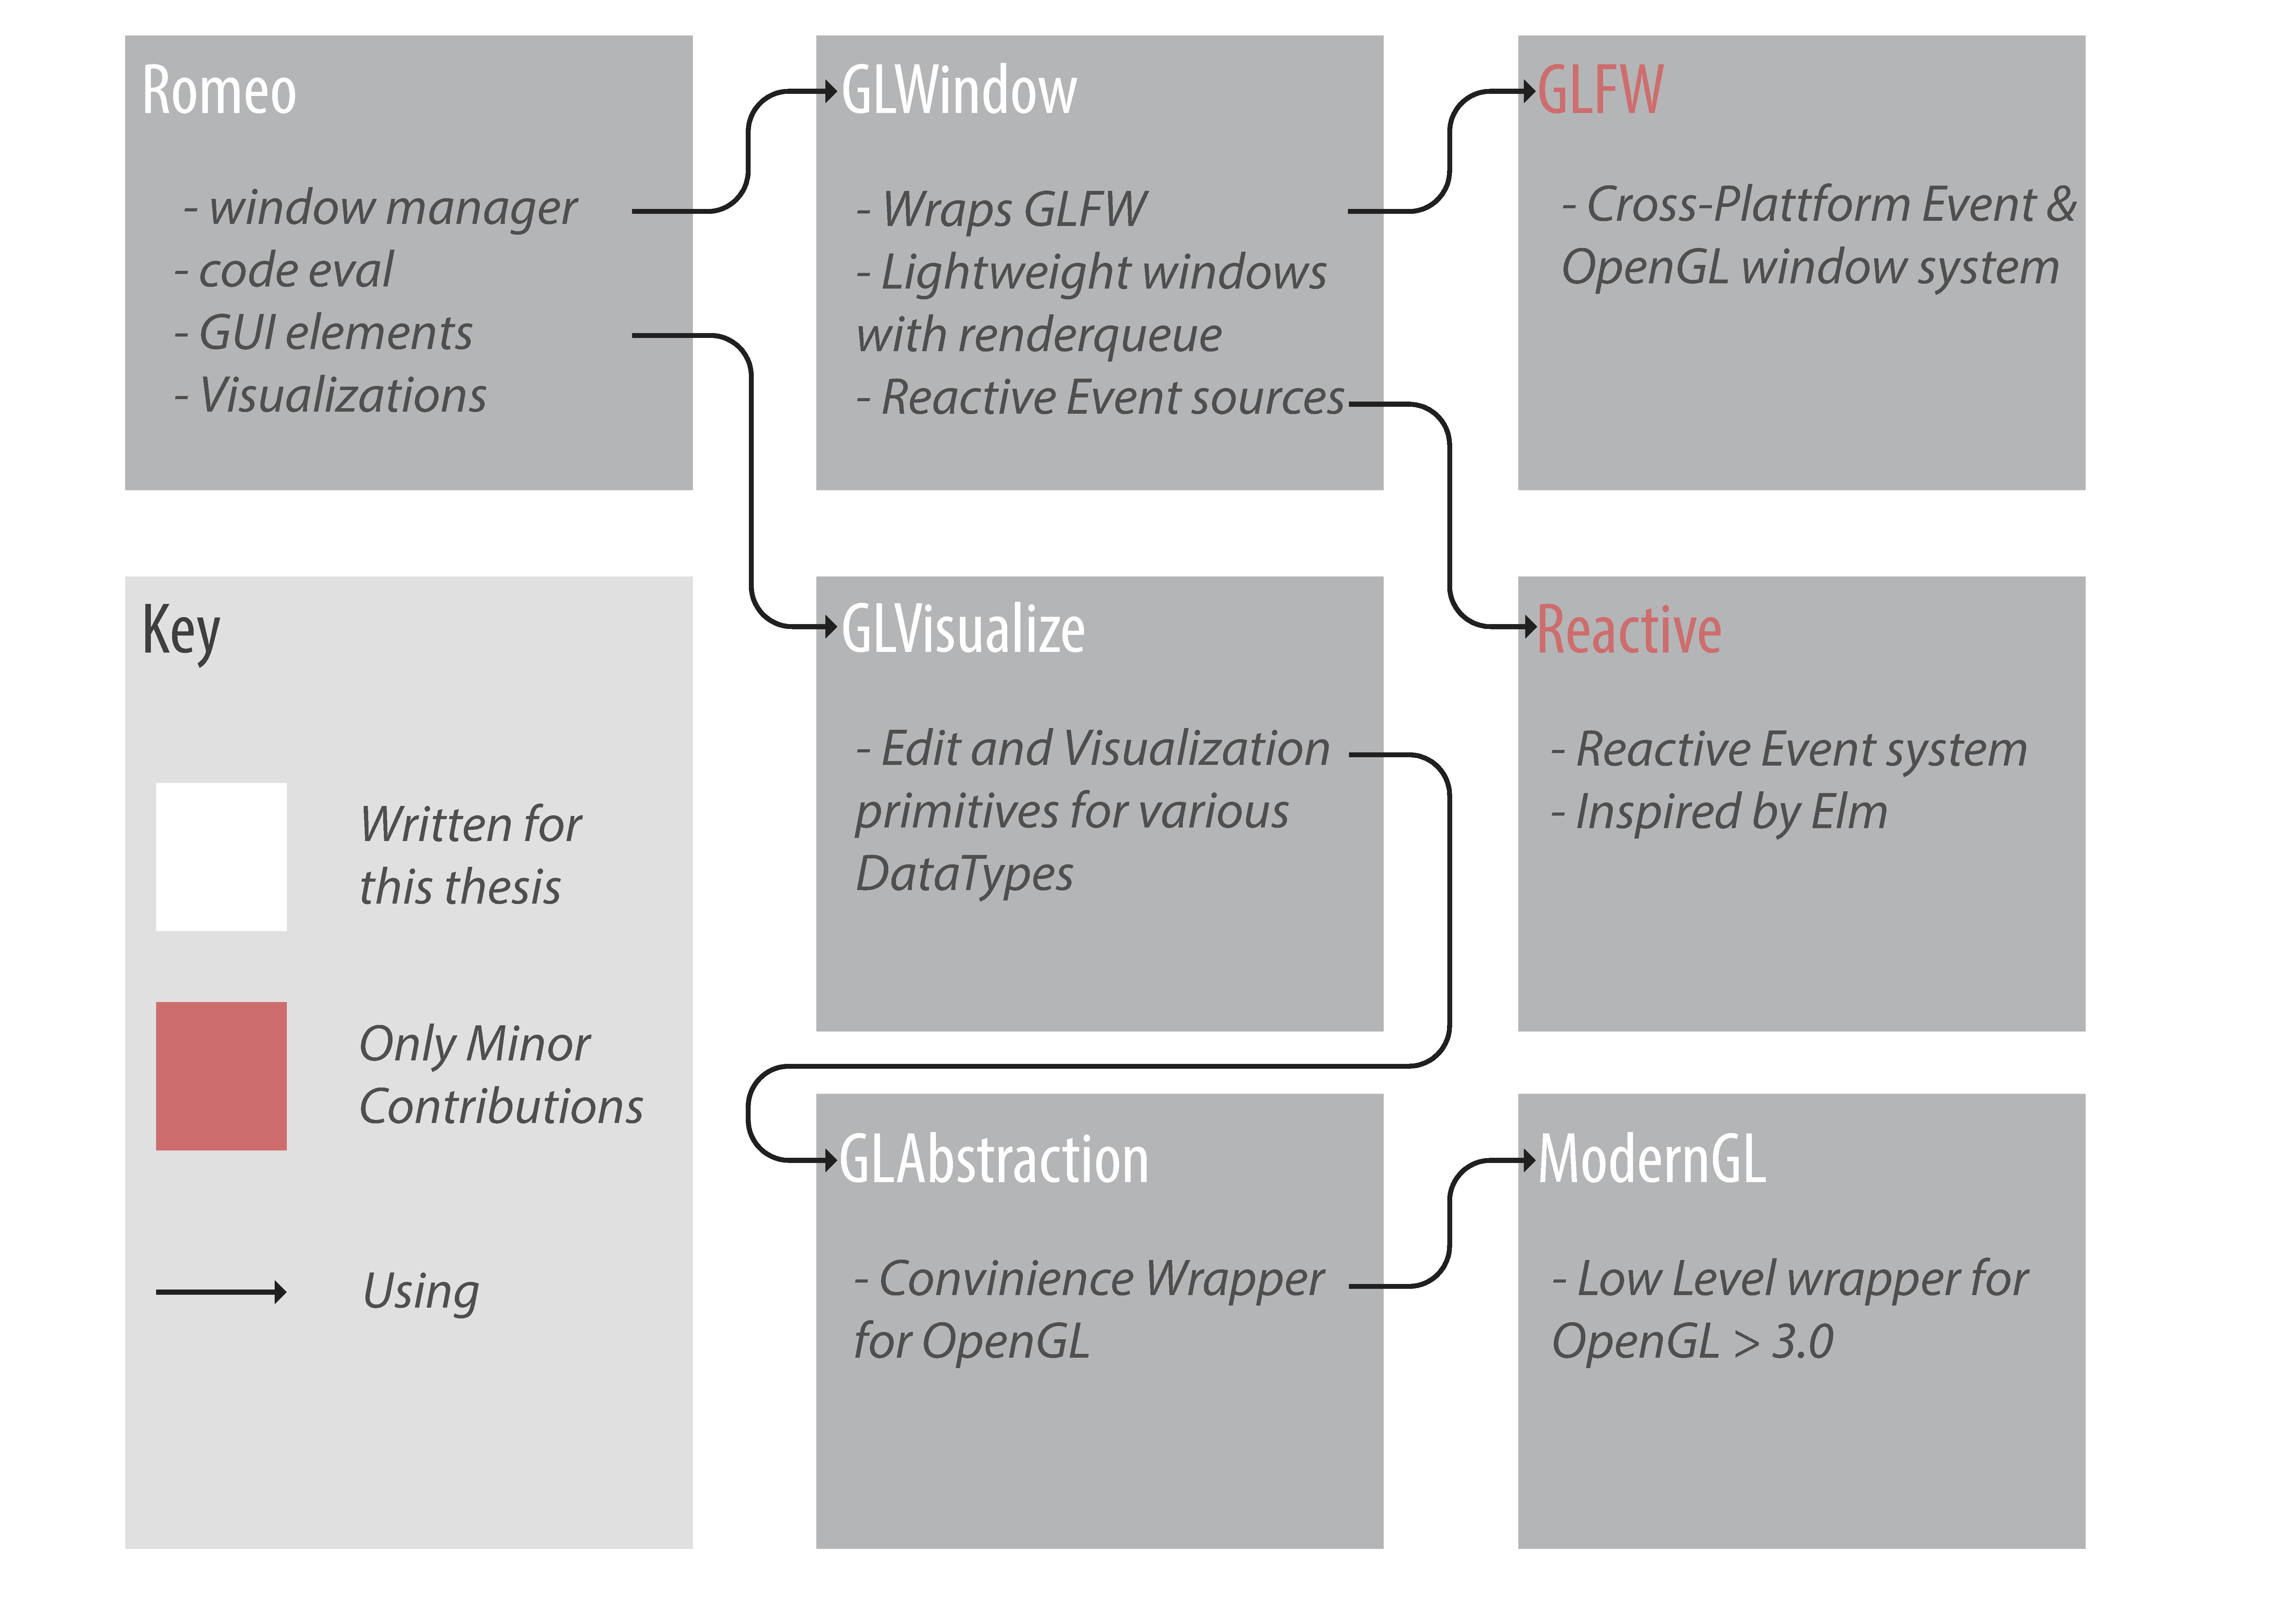
\includegraphics[width=0.9\linewidth]{graphics/architecture.pdf}
    \captionof{figure}[Architecture]{Main modules used in Romeo and their relation (simplified).}
    \label{fig:architecture} 
\end{minipage}


This chapter is about the implementation of Romeo.
The Romeo package itself is small and just defines the high-level functionality of the editor.
This includes window layout and connecting all the different event sources to create the wanted behavior.
To do this, Romeo relies on a multitude of packages, which step for step abstract away the underlying low-level code that is used to do the window creation and rendering.
As you can see in figure \ref{fig:architecture}, Romeo uses GLVisualize for creating \ac{GUI} elements and the visualisations. 
The code evaluation is done via Julia build-in functions.
Windows are managed with GLWindow. GLWindow creates an OpenGL window with the help of GLFW and converts all window events into Reactive's signals. It also offers a very simple render queue, for rendering graphics attached to a window.
Reactive signals are not only used as the event sources, but are also the main abstraction for time varying values in GLVisualize.
GLVisualize is the main package offering the rendering functionality and the editor widgets like text fields and sliders.

For rendering GLVisualize relies on GLAbstraction, which defines a high-level interface for ModernGL.
ModernGL does the \ac{OpenGL} function loading and exposes all the function and Enums definitions from \ac{OpenGL} with version higher than 3.0.
Like already pointed out in the requirements, special care has been taken to make all modules self sufficient. 
Every single package can be used for other applications, which allows for higher flexibility and a broader user base.


\subsection{Event System}

The event system was challenging to integrate for several reasons.
First of all Reactive is a functional event system, while \ac{OpenGL} relies heavily on global states, which are two perpendicular concepts.
Also, it does not allow to rearrange the event tree. 
In other words, you can not create sub trees in advance and then fuse them together at run time.

\subsection{ModernGL}
\ac{OpenGL} is implemented by the video card vendor and is shipped via the video driver, which comes in the form of a C library.
The challenge is, to load the function pointers system and vendor independent. 
Also one further complication is, that depending on the platform, 
function pointer are only available after an \ac{OpenGL} context was created and may only be valid for this context. \cite{wgl}
This problem is solved, by initializing a function pointer cache with null and as soon as the function is called the first time the real pointer gets loaded.

The OpenGL function loader from ModernGL has undergone some changes over the time.
Starting with a very simple solution, there have been pull requests to include better methods for the function loading.
The current approach in ModernGL master was not written by myself, but by the Github user aaalexandrov.
Before aaalexandrov’s approach, the fastest approach would have used a pretty new Julia feature, named staged functions.
It should in principle yield the best performance as it compiles a specialized version of the function when it gets called for the first time. This is perfect for OpenGL function loading, as the pointer to the function can only be queried after an OpenGL context has been created. When the staged function gets called the pointer can be queried and gets inlined into the just in time compiled function.

Staged functions only work with the newest Julia build, which is why aaalexandrov’s approach was used in the end.


\subsection{GLAbstraction}
GLAbstraction is the abstraction layer over ModernGL.
It wraps \ac{OpenGL} primitives like Buffers and Textures in Julia objects and hooks them up to Julia's garbage collector.
Additionally, it implements convenient functions to load shader code and it makes it easy to feed the shader with the correct data types.
Besides supplying an abstraction layer over \ac{OpenGL}, it also offers the linear algebra needed for the various 3D transformation and camera code.
Building up on that, it defines a signal based perspective and orthographic camera type.

\subsection{GLWindow}
GLWindow is a lightweight wrapper around GLFW.
It mainly offers a screen type, which contains signals for all the different GLFW events. 
It also offers a hierarchical structure for nesting screens.
All the screen areas are signals, which makes it easy to change the screen area. 
This makes it simple to implement windows that react to changing the size of the windows or resized objects.


\subsection{GLVisualize}

\vspace{1em}
\begin{minipage}{\linewidth}
    \centering
    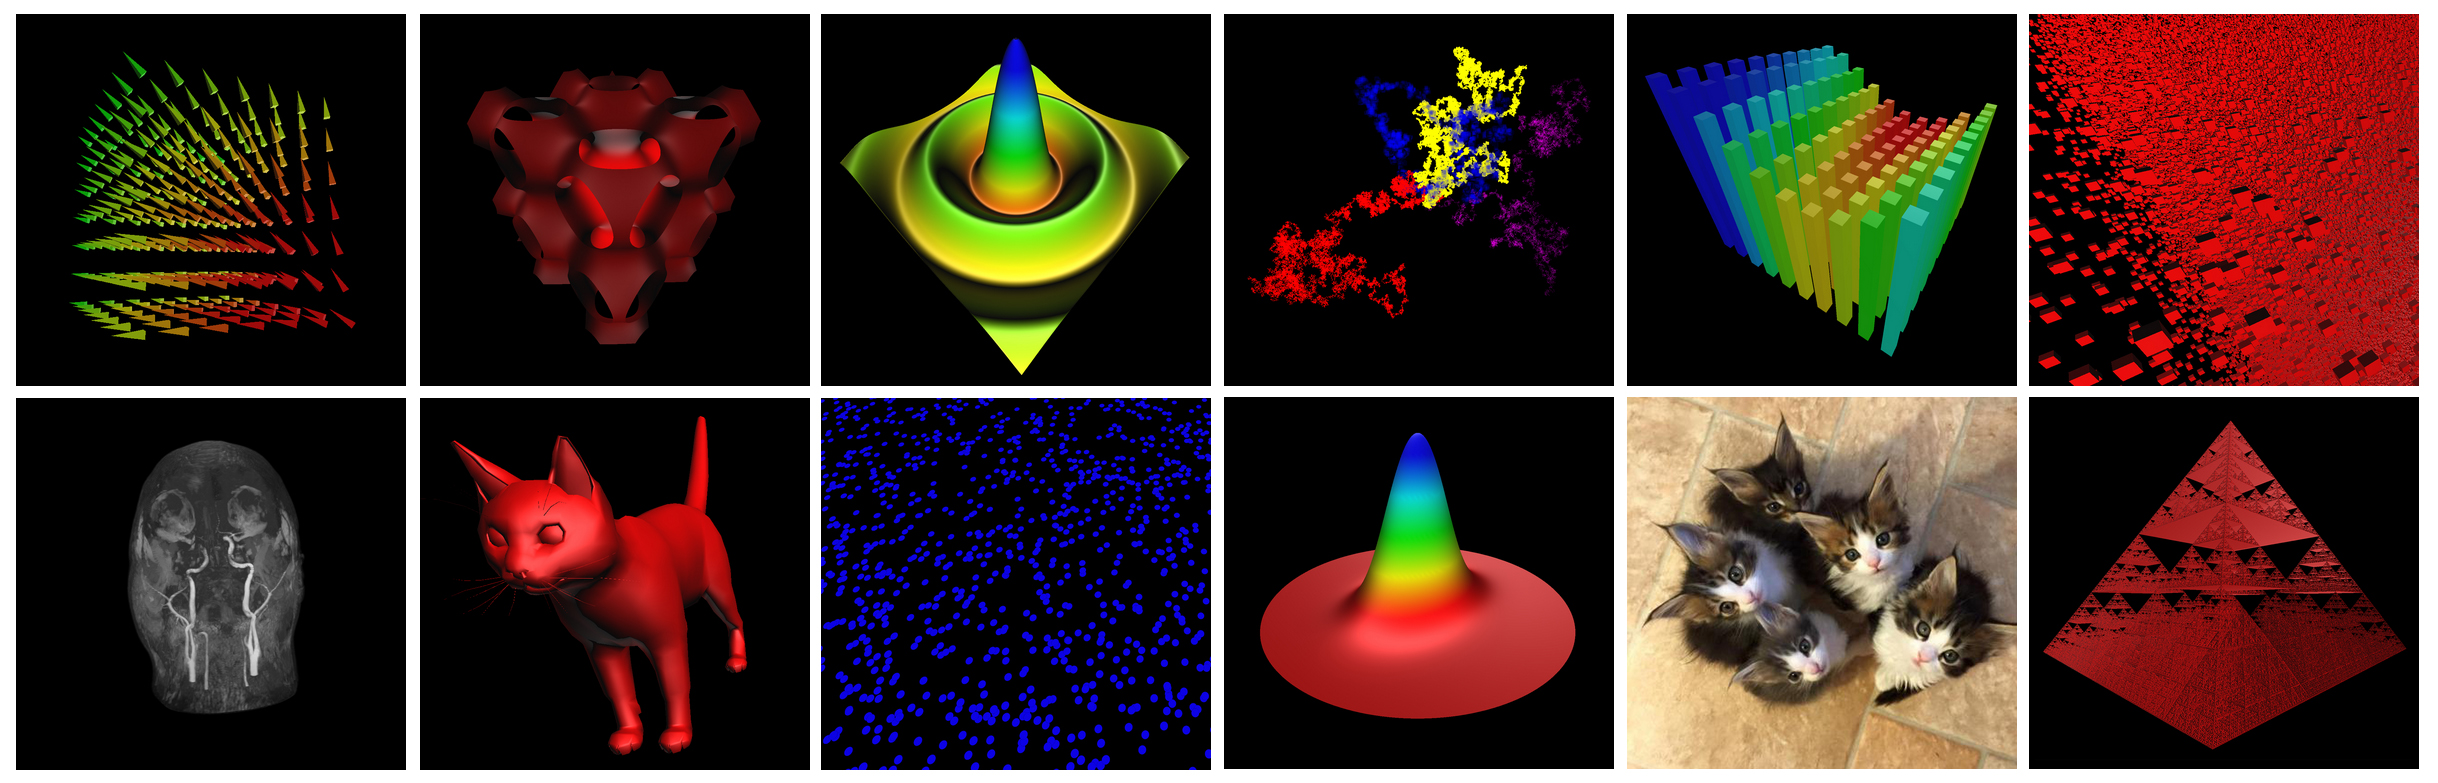
\includegraphics[width=0.9\linewidth]{graphics/glvisualize.jpg}
    \captionof{figure}[Visualisations]{Different visualizations rendered with GLVisualize.}
    \label{fig:glvisualize}
\end{minipage}

GLVisualize implements the main functionality of this library.
It structure is quite simple. 
It relies as much as it can on common Julia data types and creates specialized visualizations for them via dispatch.
So instead of offering differently named functions for different visualizations, there is just one function with lots of methods for different types.
This has two advantages.
First, it makes it very easy to use for visual debugging, as any value can be displayed immediately without any user interaction.
Secondly, the user does not have to remember or lookup the function name, as long as there is a default visualization for the type he is working with.
The next design goal was to make this fit for dynamic data, which resulted in relying on as little transformation of the data as possible and directly transferring it to the GPU.
Depending on the complexity of the visualization, this means the visualization can be updated with as little overhead as possible.

The interface to create visualizations is very simple and only consists of three functions:
\begin{lstlisting}
Dict{Symbol, Any}     = visualization_defaults(data::Union(Signal{T}, T), style::Style) # returns a dictionary of parameters
RenderObject 		  = visualize(data::Union(Signal{T}, T), style=Style{:default}; parameters...) # returns an object which can be directly rendered
RenderObject, Signal  = edit(data::Union(Signal{T}, T), style=Style{:default}; parameters...) # returns an RenderObject and signal which outputs the changed values
\end{lstlisting}

With this simple interface, the following data can be visualized:

\begin{itemize}
	\item Text (Vector of Glyphs)
	\item Height fields with different primitives (Matrix of height values)
	\item 3D bar plots (Matrix of height values)
	\item Images (Matrix of color values)
	\item Videos (Vector of Images)
	\item Volumes (3D Array of intensities)
	\item Particles (Vector of Points)
	\item Vector Fields (3D array of directional Vectors)
    \item Colors (Single Color values)
\end{itemize}

All of these can be integrated into the same scene and it is possible to change their parameters interactively.
These interactions can be purely programmatically, or via the widgets from the edit function.
It calls the visualize function to render the data type and then registers appropriate events to update the data.
Take a look at the text edit function.
It first uploads the text to video memory and sets up the functionality to visualize it, and than updates the text data on the GPU according to the cursor position and keyboard input.

Up to now, there is an edit function available for strings, colors, numbers, vectors and matrices.


\subsubsection{Particle Rendering}
Most of the visualizations in GLVisualize are realised via instancing a mesh primitive.
So the barplot is nothing else than a cube placed in a grid, with scaling informations that get applied to every individual cube. The surface plot is a quad or any other 2D mesh spaced across a grid, while the vertexes are projected onto a height field. The vectorfield is a mesh placed regularly inside a cube, while the rotations from the vectorfield gets applied to this mesh. 
Even text rendering functions in the same way. The difference is just, that the particle not only holds position information, but also indexes to a texture atlas in which renderings of the glyphs are cached. So when rendering the text particles, the exact scale and image of the glyph is queried, which will then be used to render a quad with the image of the particular glyph to the screen.
The texture atlas approach was chosen, because rendering a high quality vector graphic is very time consuming, especially if the description of the font is only available as a bezier spline.% Closer description, or source?!
All particles are rendered via OpenGL's instanced rendering API, which allows to render millions of particles with only one draw call and very little memory usage, as the geometry of the particle just needs to be uploaded one time.
The geometry of the particle will then be rendered x times. For every individual particle additional information like color, position, scale and so forth can be queried from the fragment or vertex shader.
Theís additional information can be stored in uniform buffers, uniform arrays or textures. Textures have been choosen for this thesis, as they offer the greatest support among devices and are easy to use. In the future, other approaches can be implemented, gaining more performance or flexibility.
The texture approach has the disadvantage that 1D textures offer maximum sizes between 1024 and 8192 elements, so for greater amounts of particles the 1D vector had to be transformed to a 2D texture.



\subsubsection{Vector Graphics Rendering}
\subsubsection{Volume Rendering}


\subsection{Romeo}
So far Romeo just consists of one file with 500 lines of code. It just defines some simple text field, a search field, and a visualize and edit window.
The texts gets evaluated as Julia code as soon as it changes. Like this, the text field acts like a very simple \ac{REPL}.
Via the search field, you can execute simple Julia statements and the results will be displayed in the visualize window, while all parameters can be edited via the edit window.
This means, if you type in a simple variable, the variable will be visualized. But you can also search and transform a variable via simple Julia terms.